\documentclass[../main/main.tex]{subfiles}


\begin{document}

\section{February 26th, 2021}
\subsection{Humanistic Perspective}\index{humanistic perspective}
The humanistic perspective has an emphasis on free will and achieving self-fulfilment.
\subsubsection{Carl Rogers' Conditions of Worth}
\begin{definition}[\vocab{Positive Regards}] warmth, affection, love and respect.\index{positive regards}
\end{definition}
\begin{definition}[\vocab{Conditions of Worth}]\index{conditions of worth}
\end{definition}
There are two conditions where a person will receive conditions of worth:
\begin{description}
  \item[Conditional Positive Regard:] Positive regard given when providers' wishes fulfilled
        \begin{example}
Becoming a doctor because parents want is an example of conditional positive regard.
        \end{example}
        However, people are unable to self-actualize with conditional positive regard. As such, it is not ideal.
\item[Unconditional Positive Regard:] Unconditional love and acceptance of an individual by another person.
\end{description}
\subsection{Evaluation of the Humanistic Perspective}
\subsubsection{Contributions}
\begin{itemize}
  \item Reinforces the idea of free-will
        \item Highlights unique human qualities
\end{itemize}
\subsubsection{Limitations}
\begin{itemize}
\item Unable to identify and explain age-related developmental changes, similar to the behavioral perspective.
\end{itemize}

\subsection{Biological Perspective}
There are three biological theories, we will look at:
\begin{itemize}
\item Behavior Genetics
        \item  Evolutionary Theory
        \item Ethology
\end{itemize}

\subsubsection{Behavior Genetics}\index{behavior genetics}
Our individual differences are determined by heredity (genes). This means that related people, such as children and parents have similar traits influenced by genes.\\

A child's pattern of inherited quality can influence how she behaves with others.
\begin{example}
  A child with a higher intellect would seek out challenging problems, resulting in the parent giving them more support their development. Thus, there is a biderictional influence on the child's genes and their environment.
\end{example}

\subsubsection{Adoptive and Twin Studies}
Infants who were adopted early in infancy were studied to see whether there is resemblance between adopted children and both their biological and their adoptive parents. If the adopted children has stronger resemblance with their biological parents, then biological factors play a large role. Figure \ref{2-26-bio} shows the result of one such study.

\begin{figure}[htpb]
  \centering
  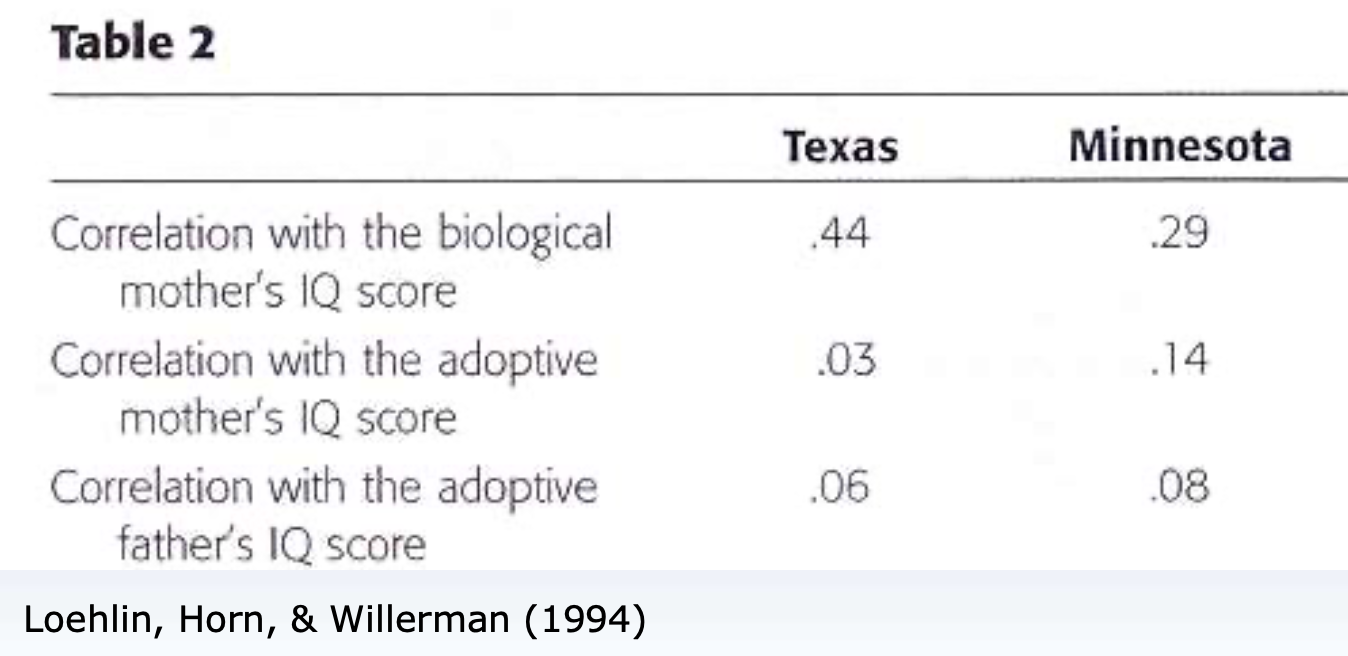
\includegraphics[width=0.8\textwidth]{2-26-bio}
  \caption{Result of an Adoptive Study on Intelligence}
  \label{2-26-bio}
\end{figure}
Adoptive studies found the biological factors are important in shaping an infant's intelligence. Later on, they found that it is interaction between the biological factors and the child's environment. Nonetheless, genetics does play a role.\\

Other studies also looked at identical and fraternal twins. If sets of identical twins are more like each other on a trait than fraternal twins, then it suggests the biological factors do play a role in the development of that trait. Studies, such as Figure \ref{2-26-bio2}, found that this is indeed the case.

\begin{figure}[htpb]
  \centering
  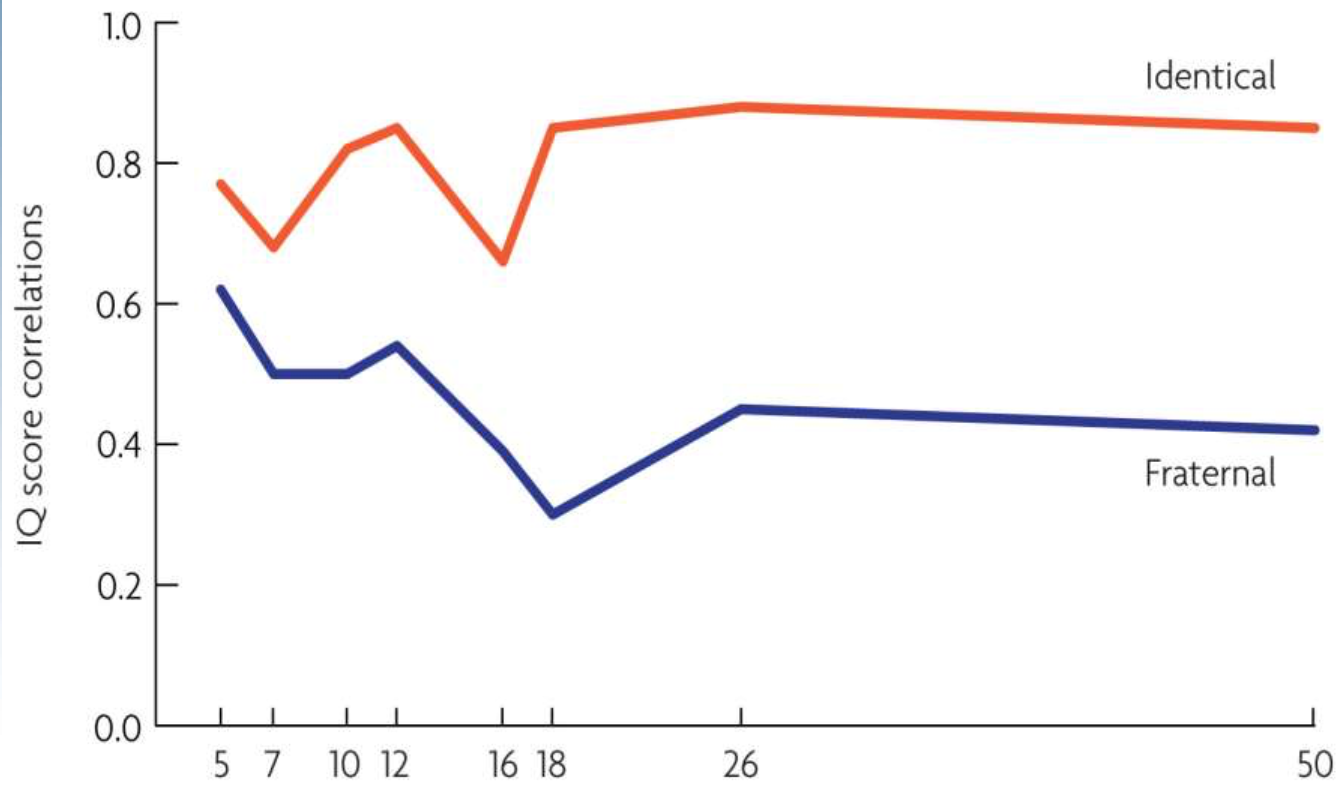
\includegraphics[width=0.8\textwidth]{2-26-bio2}
  \caption{Results of a Twin Study on Intelligence}
  \label{2-26-bio2}
\end{figure}

\subsubsection{Evolutionary Theory}\index{evolutionary theory}
Genes play a central role in an individual's adaptation to environmental demands. Evolutionary Theory looks at how these traits are passed on/ influenced by ancestry. There are three main evolutionary forces:
\begin{description}
  \item[Survival of the Fittest:] Species with traits better adapted to their environment survive and reproduce
    \item[Natural Selection:] Through reproduction, more adaptive traits are selected to be passed onto future generations by genes.
    \item[Evolved Mechanisms:] Behaviors developed to solve problems in adapting to an earlier environment which may no longer serve a useful purpose.
        \begin{remark}
Women having a distaste in some foods while pregnant is an example of an evolved mechanism.
        \end{remark}
\end{description}

\subsubsection{Ethology}\index{ethology}
\begin{definition}[\vocab{Ethology}]
The scientific study of animal behavior.
\end{definition}
The reason why ethology is important is:
\begin{itemize}
  \item Sometimes it is not possible to perform some studies on human being.
        \item Animal behaviors can sometimes be similar to human behaviors.
\end{itemize}
One famous Ethologist is Kinrad Lorenz who looked at birds. In particular:
\begin{description}
  \item[Imprinting in Birds:] Imprinting is when the bird becomes emotionally attached to the first moving object.
        \begin{example}
One group of ducklings were exposed to their biological mother at birth. The other group was exposed to Lorenz himself. The birds in the latter group were attached to Lorenz as if he was their caregiver.
        \end{example}
\end{description}

Imprinting in birds is generalized to \vocab{parent-infant attachment} in human. However, the development of attachment is slightly different, as it take a while for an infant to be attached to their primary caregiver.

\subsection{Evaluation of the Biological Perspective}
\subsubsection{Contributions}
\begin{itemize}
        \item Shows the importance of genetic factors, with strong empirical evidence.
\end{itemize}
\subsubsection{Limitations}
\begin{itemize}
        \item Ignores the impact of environmental influences.
\end{itemize}

\subsection{Conclusion on Theories of Development}

We have seen 5 different theoretical perspectives. Which one should we use to model development? There is no single theory that can explain everything in human development. Many of them have some element of truth, however no single theory is perfect. Nowadays there are 3 major ideas:

\begin{itemize}
  \item Developmental influences are \textbf{bidirectional}.
\item Both nature and nurture are important in a person's development. Instead of asking which is more important, we should ask how they interact to affect development.
  \item There is no single theory of development. Instead we should combine them. This is called eclecticism.
\begin{definition} [\vocab{Eclecticism}] The combination of different theories in explaining human development.
\end{definition}
\end{itemize}

\subsection{Reading - Chapter 1}

\subsection{Cognitive Development}\index{cognitive development}
\begin{definition}
\vocab{Cognitive development} refers to the process by which a child's understanding of the world changes as a function of age and experience.
\end{definition}
In this chapter, we will look at two theories in cognitive development:
\begin{itemize}
\item Piaget's Cognitive Development Theory
        \item Information Processing Theory
\end{itemize}
\subsection{Piaget's Cognitive Development Theory}\index{Piaget's cognitive development theory}
According to Piaget's theory, one of the most importance concept is that of scheme/schema.
\begin{definition}
\vocab{Scheme/schema} refers to the beliefs, cognition, and ideas about things
\end{definition}
\begin{example}
We all have a idea (schema) of what a dog is, e.g. cute, pet, etc. However, how did we develop this scheme?
\end{example}
There are two main ways people develop scheme:
\begin{description}
  \item[\vocab{Organization:}] The process of deriving generalizable schemes from specific experiences.
        \begin{example}
Prior experience with dogs might influence our development of our schema for dogs.
        \end{example}
  \item[\vocab{Assimilation}] The process of using schemes to make sense of experiences.
        \begin{remark}
Our scheme of dogs will affect how we interact with dogs.
        \end{remark}
\end{description}
Our schema may also change across time through the following processes:
\begin{description}
  \item[\vocab{Accomodation:}] Changing a scheme to incorporate new information. We might refine our skills and knowledge
        \begin{example}
          After interacting with a therapy dog, we might change our scheme of dog.
        \end{example}
  \item[\vocab{Equilibration:}] Balancing assimilation and accommodation.
\end{description}
Piaget's has proposed different stages across a person's lifespan:
\begin{itemize}
\item Sensorimotor stage (birth-2 years)
\item Preoperational stage (2-7 years)
\item Concrete operations stage (7-12 years)
\item Formal operations stage (12 years-adulthood)
\end{itemize}
\begin{definition}
[\vocab{Operations}] mentally acting on objects.
\end{definition}
These stages covers development from action-, physical reality-based thinking to abstract, symbol-based thinking.\\

According to Piaget, this sequence of stages is programmed in our genes (maturation). As such, this theory has aspects of both nature and nurture:
\begin{itemize}
  \item Nature - brain development and maturation.
        \item Nurture - social transmission and experience,
        \begin{definition}
Social transmission is the information the child receive from others.
        \end{definition}
        \begin{remark}
In particular, Piaget believes that education affects our speed of development greatly.
        \end{remark}
\end{itemize}
Both nature and nurture affects the speed of development of a child.
\begin{remark}
All individuals will reach the formal operations stage, but some might achieve this stage earlier or later.
\end{remark}

\subsubsection{Sensorimotor Stage}
\begin{itemize}
\item Infants acquire knowledge of the world from the physical actions they perform on the environment
\item Infants progresses from reflective actions at birth to the emergence of symbolic thoughts towards the end.
\end{itemize}
There are certain substages of sensorimotor stage:
\begin{description}
  \item[Reflexes (birth-1 month):] Automatic body reactions to external stimulations (from genes). This allows the infant to get information about the outside world.
        \begin{remark}
Some reflexes persist into adulthood, other gradually disappear in the first year of life
        \end{remark}
        There are a few common reflexes that will disappear gradually:
        \begin{itemize}
          \item Rooting reflexes: turning head to the source of stimulus near the mouth. This will allow the baby to find a source of food, e.g. milk bottle.
          \item  Babinski reflex: Stroking the bottom of a foot would cause the toes to stretch out. This will allow the baby to better support themselves when they stand up.
                \item Grasp reflex: grasping objects. This will allow the baby to support themselves.
        \end{itemize}
        Some of these reflexes are important to motor development.
  \item[Primary circular reactions (1-4 months):]
        Primary refers to being related to the child's body, circular refers to repetitive.
        \begin{example}
Sucking on their thumb is an example of a primary circular reaction.
        \end{example}
        Usually babies are not able to do this right away. Thus, they undergo trial-and-error learning by repeating until they become successful or become a habit.

  \item[Secondary circular reactions (4-8 months):] Again, the infant will repeat some actions, but this time, they repeat some actions in order to trigger a reaction in the environment.
        \begin{example}
A baby coo-ing is one example of a secondary circular reaction, as people will react positively to the baby coo-ing. Thus, the baby will repeat this.
        \end{example}
    \item[Coordination of secondary circular reactions (8-12 months):] Now the baby will coordinate/combine more than one secondary circular reaction to achieve a goal. In this stage, the baby will demonstrate \vocab{goal-directed behavior}.
        \begin{example}
Suppose a baby wants to grab the teddy bear behind other toys. In order to reach the teddy bear, they will move away the other toys.
        \end{example}
        In this stage, the baby achieves a few developmental milestones:
        \begin{itemize}
          \item \textbf{Imitation} -
                The baby is able to imitate other people, e.g. facial expressions.
          \item \vocab{Object Permanence} - The baby has an understanding that objects not in their view, cannot be heard or touched, still exist.
                \index{object permanence}
                \begin{example}
One study tested object permanence in infants by hiding a toy. Until the age of about 9 months, children will make no attempts to locate hidden toys. Soon after that age, they will actively search for the hidden objects.
                \end{example}

                Object permanence indicates the emergence of mental representation of objects.
        \end{itemize}
\vocab{A-not-B-error} is a phenomenon whereby infants search successfully for an object hidden in one position (A), but when the object is hidden in a new position (B), they continue to search back in the old location. Infants of 12 months or younger typically make this error.
            \begin{remark} This phenomenon indicates an incomplete schema of object permanence.
                \end{remark}
                There are a few explanations for this A-not-B phenomenon:
                \begin{itemize}
                  \item Response preservation - might just be a habit of searching for the object at position A (similar to absent minded adults).
                  \item Proactive interference - when there is interference in memory. The information of the object being at the two locations might be mixed up.
                  \item Frontal cortex immaturity - the frontal cortex of the child might not be developed enough.
                        \begin{remark}
The frontal cortex is responsible for the planning and execution of actions. These actions are called \vocab{executive functions}.
                        \end{remark}
                \end{itemize}
  \item[Tertiary circular reactions (12-18 months):] Here the infant tries to produce novel reactions with variations of previous actions. The child is able invent new behaviors.
        \begin{example}
Instead of stepping on a duck, they
        \end{example}
  \item[Beginning of representational thoughts (18-24 months):] The child is able to use symbols (e.g. images, words, and drawings) to represent objects or events.
\begin{remark}
  Another developmental milestone is deferred imitation - the ability to imitate an action at a later time.
\end{remark}
\end{description}
In summary in the sesorimotor stage, infants use information from their senses and motor actions to learn about the world.




\end{document}
